%!TEX root = ./thesis-main.tex
\chapter{Implementazione e Verifica}

\section{Componenti grafici}
Lo sviluppo web moderno trae benefici significativi da framework che semplificano la creazione di applicazioni web. Tutte le componenti grafiche all'interno di questo progetto sono state sviluppate attraverso l'utilizzo del framework open-source \textit{KVision}\footnote{\url{https://kvision.gitbook.io/kvision-guide/}}, che permette agli sviluppatori di costruire interfacce web moderne senza utilizzare HTML, CSS o JavaScript. Le interfacce vengono assemblate attraverso la composizione di oggetti pronti all'uso, seguendo un paradigma paragonabile a quello dichiarativo. Il risultato sono gerarchie di componenti che possono essere usate come blocchi costituenti. In aggiunta, \textit{KVision} presenta supporto integrato per gli store Redux (esplorati in \cref{section:state-management}), per le icone Font Awesome, per Bootstrap e molto altro. Questa libreria sfrutta puramente le capacità del linguaggio Kotlin (compilato per target JS), specialmente con l'utilizzo di \textit{type safe builders}, implementati attraverso \textit{extension functions}. Quello offerto da \textit{KVision} è di fatto un \ac{DSL}, di cui si è fatto ampiamente uso.
Nel \cref{lst:graphic-comp-declaration} è illustrata, a scopo esemplificativo, una versione riadattata della definizione della struttura del contenuto principale della pagina web.

\lstinputlisting[float=htb, language=KVision, label={lst:graphic-comp-declaration}, caption={\ac{DSL} KVision per la struttura del contenuto principale della pagina},captionpos=b]{listings/Content.kt}

Per la maggioranza degli elementi dichiarabili in HTML, esiste una classe corrispondente offerta da \textit{KVision}. Da qui deriva la natura dichiarativa nello sviluppo delle componenti grafiche. Questo avviene grazie all'utilizzo di \textit{extension functions}, funzionalità caratteristica del linguaggio Kotlin che permette di aggiungere nuovi comportamenti a classi esistenti senza dover ereditare da esse o modificarle direttamente. In questo caso, ciò significa che per un elemento del \ac{DOM} come \texttt{div}, il framework fornisce la classe \texttt{Div} alla qual è stata aggiunta l'\textit{extension function} \texttt{div()} che funge da \textit{builder}. L'invocazione di quest'ultima evita la memorizzazione dell'istanza della componente in una variabile separata, e la successiva aggiunta manuale alla lista di figli della classe padre che li contiene.
Nel \cref{lst:graphic-comp-declaration} sono stati creati componenti custom che estendono la classe \texttt{SimplePanel} (classe base per un semplice pannello rappresentabile nella pagina). Si parla di \texttt{SimulationContext}, \texttt{SimulationIndicators} e \texttt{NodeProperties}, come indicato nella sezione \ref{section:page-structure}. In questo caso sono stati aggiunti manualmente come componenti figli delle rispettive classi padre, tramite il metodo \texttt{add()}. Sarebbe stato possibile aggiungere a queste classi una \textit{extension function} per creare un builder. Ogni volta in cui sarebbe stato necessario dichiarare più volte questo tipo di oggetto in diverse parti dell'applicativo, sarebbe bastata una invocazione come nel \cref{lst:graphic-comp-declaration-ext}. In questo caso non era strettamente necessario, perché queste componenti vengono istanziate una volta sola.

\lstinputlisting[float=htb, language=KVision, label={lst:graphic-comp-declaration-ext}, caption={Uso di \textit{type-safe} builders},captionpos=b,captionpos=b]{listings/Content_ExtensionFunction.kt}

La manipolazione degli elementi all'interno di un contenitore in una pagina web risulta essere molto onerosa se si fa uso di HTML e CSS puro. La convenienza di utilizzo di questo framework risalta anche nell'esistenza di elementi pronti all'uso come \texttt{hPanel} e \texttt{vPanel}, due costrutti che dispongono, rispettivamente, in orizzontale e in verticale gli elementi aggiunti al loro interno. La disposizione degli oggetti all'interno di questi layout è facilitata perché quest'ultimi rispettano le specifiche della recommendation \textit{CSS Flexible Box Layout} \footnote{\url{https://www.w3.org/TR/css-flexbox/}}.

Inutile dire che la libreria utilizzata offre una vasta gamma di costrutti e metodi che semplificano notevolmente lo sviluppo di interfacce utente, contribuendo così a migliorare l'efficienza complessiva del processo di sviluppo.

\section{Integrazioni di operazioni GraphQL}
Nella sezione \ref{section:graphql-connection} sono stati illustrati i motivi dietro all'utilizzo di un unico punto di accesso per l'esecuzione delle \textit{query}, \textit{mutation} e \textit{subscription} all'interno dell'applicativo. A questo scopo i \textit{Singleton} \texttt{EnvironmentApi} e \texttt{SimulationControlApi} raggruppano al loro interno funzioni che avviano operazioni sul modello fra loro correlate.
Come suggerisce il nome, il primo presenta tutte le operazioni effettuabili sull'ambiente della simulazione, mentre il secondo contiene quelle legate al controllo della simulazione.
Per illustrare meglio come avvengono le operazioni sul server GraphQL, viene presentata l'implementazione della query che reperisce lo stato corrente della simulazione.
\begin{enumerate}
	\item È stata definita l'operazione voluta, come riportato nel \cref{lst:graphql-status-query}. 
	\lstinputlisting[float=htb, language=Kotlin, label={lst:graphql-status-query}, caption={Query GraphQL per il recupero dello stato corrente della simulazione},captionpos=b,captionpos=b]{listings/SimulationStatus.graphql}
	\item Al momento della compilazione del progetto, viene generata dalla libreria \textit{Apollo} \footnote{\url{https://github.com/apollographql/apollo-kotlin}} la classe Kotlin \texttt{SimulationStatusQuery} dentro al modulo \texttt{graphql} (pacchetto denominato come \textit{GeneratedSources}, vedi \ref{item:generated-sources}).
	\item La funzione \texttt{getSimulationStatus()} del \cref{lst:graphql-query-execution}, esegue la query tramite l'avvio di un thread asincrono, in modo che questa chiamata non influisca sul thread di rendering principale della \ac{UI}.
	\lstinputlisting[float=htb, language=Kotlin, basicstyle=\ttfamily\footnotesize, label={lst:graphql-query-execution}, caption={Esecuzione asincrona della query SimulationStatus},captionpos=b,captionpos=b]{listings/SimulationStatusQueryExec.kt}
	\item La query può essere chiamata in qualsiasi momento tramite la funzione \newline \texttt{callGetStatus()} (\cref{lst:graphql-query-call}).
	\lstinputlisting[float=htb, language=Kotlin, label={lst:graphql-query-call}, caption={Chiamata per il prelievo dello status della simulazione},captionpos=b,captionpos=b]{listings/SimulationStatusQueryLaunch.kt}
	
\end{enumerate}
La natura e il tipo di ritorno di queste funzioni varia in base al tipo di operazioni effettuate, ovvero:
\begin{itemize}
	\item \textbf{query} e \textbf{mutation}: per questo tipo di operazioni ci si aspetta un unico valore di ritorno. L'esecuzione di queste procedure avviene in modo asincrono attraverso l'utilizzo del costrutto \texttt{async()}, servito dalla libreria Kotlin \textit{kotlinx.coroutines}\footnote{\url{https://kotlinlang.org/docs/coroutines-guide.html}}. Il risultato viene restituito dal server una volta che la richiesta ha avuto successo. L'attesa del completamento dell'esecuzione della funzione che esegue la query avviene invocando \texttt{await()}. Non a caso, questo tipo di funzioni possono essere sospese. Da qui il motivo per il modificatore d'accesso \texttt{suspend}.
	\item \textbf{subscription}: diversamente da quanto descritto per \textit{query} e \textit{mutation}, l'esecuzione di una \textit{subscription} fornisce come risultato un oggetto di tipo \texttt{Flow}, di cui si esamina il comportamento in \cref{subsection:node-representation}.
\end{itemize}

\section{Gestione dello stato}\label{section:state-management}
Il framework \textit{KVision}, oltre a fornire strumenti e metodi di programmazione molto robusti e versatili, dona la possibilità di usare tutta la capacità della libreria di \textit{Redux}\footnote{\url{https://redux.js.org/tutorials/essentials/part-1-overview-concepts}}, una libreria open-source per la gestione dello stato delle applicazioni JavaScript. Il fulcro di questa libreria consiste nel cosiddetto \textit{store}, un archivio centralizzato per uno stato che deve essere condiviso in tutta l'applicazione, attraverso l'utilizzo di regole che garantiscono che lo stato possa essere aggiornato solamente in modo prevedibile. Analizziamo ora il funzionamento della gestione dello stato introducendo tutti i concetti chiave: 
\begin{itemize}	
	\item \textbf{State}: \textit{``The source of truth that drives our app''}, in altre parole, dati o insieme di dati che influenzano il comportamento o l'aspetto dell'applicazione. 	
	\item \textbf{View}: una descrizione dichiarativa dell'interfaccia utente basata sullo stato attuale.
	\item \textbf{Actions}: usati per descrivere possibili cambiamenti dello stato. Sono oggetti, dotati di un campo che ne indica il tipo, incaricati a indicare l'azione che deve essere eseguita sullo store per cambiarne lo stato. Si può pensare a questo tipo di oggetti come ad eventi che riportano un certo avvenimento nell'applicazione. Di solito vengono chiamati dopo un input, ovvero quando si verifica un evento specifico nell'applicazione, come un click del mouse o quando un pulsante viene premuto.
	\item \textbf{Store (archivio)}: l'oggetto centrale che contiene lo stato dell'applicazione in un determinato momento.
	\item \textbf{Reducers}: funzioni che descrivono esattamente come deve essere cambiato lo stato, in risposta alle azioni chiamate sullo store. Come parametri di ingresso accettano lo stato corrente e l'azione che si vuole eseguire, ritornando un nuovo stato. I reducer possono essere paragonati a dei \textit{listener} che gestiscono gli eventi (\textit{actions}) in base al loro tipo.
	\item \textbf{Dispatch}: metodo di cui lo store dispone. L'unico modo per aggiornare lo stato è invocando questa funzione, passando come parametro un'azione.  A questo punto lo store può eseguire il suo \textit{reducer} e salvare il nuovo stato al suo interno. Nel momento in cui un evento viene innescato (proveniente per esempio della \ac{UI}), si vuole di conseguenza aggiornare il valore dello store.
	\item \textbf{Subscribe}: sono funzioni che permettono ai componenti grafici di ``iscriversi'' ai cambiamenti di stato dello store. Ogni volta che lo stato cambia, i componenti iscritti vengono avvisati, dando la possibilità di aggiornare la \ac{UI} in base al nuovo cambio di stato.
\end{itemize}
Insieme agli elementi appena descritti, la figura \cref{fig:redux-scheme} offre una visione più completa del funzionamento della gestione dello stato.
\begin{figure}[htb]
	\centering
	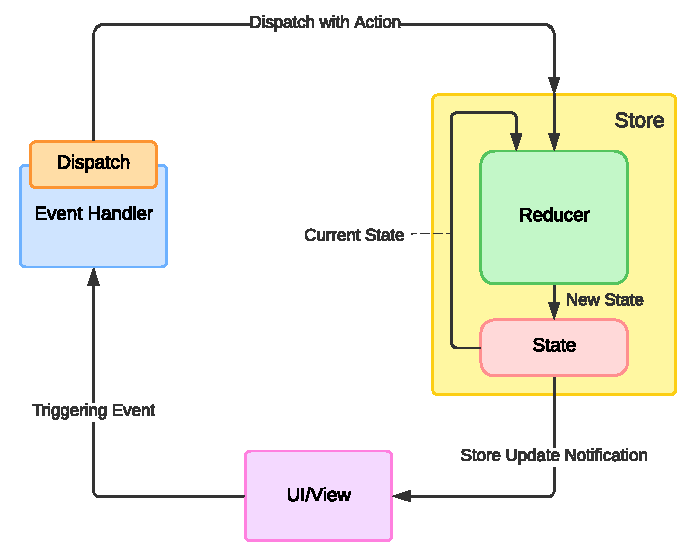
\includegraphics[scale=0.8]{imgs/Redux_Scheme.pdf}
	\caption{Funzionamento di uno store Redux}
	\label{fig:redux-scheme}
\end{figure}
Dallo schema è possibile notare come sia presente una unica direzione che collega le varie entità. Questo è dovuto al fatto che la sequenza dei passi da compiere per l'aggiornamento dello stato segue il paradigma \textbf{``one-way data flow"}.

 In particolare, per Redux si seguono quindi questi passaggi:
\begin{enumerate}	
	\item Accade un evento nell'applicazione, come un utente che fa clic su un pulsante.
	\item Viene chiamata la funzione \texttt{dispatch()}, specificando l'azione per modificare lo store Redux.
	\item Lo store esegue la funzione reducer con lo stato precedente e l'azione corrente, e salva il valore restituito come nuovo stato.
	\item Lo store notifica a tutte le parti dell'interfaccia utente che sono iscritte che lo store è stato aggiornato.
	\item Ciascun componente dell'interfaccia utente che necessita dei dati dallo store controlla se le parti dello stato di cui hanno bisogno sono cambiate.
	\item Ciascun componente che rileva che i suoi dati sono cambiati, forza un nuovo rendering con i nuovi dati, così da poter aggiornare ciò che viene mostrato sullo schermo.
\end{enumerate}
\paragraph{Stato del nodo selezionato}
All'interno dell'interfaccia grafica è possibile ottenere le informazioni di un nodo effettuando una apposita query al server GraphQL. Queste informazioni possono essere utili all'interno di tutta l'interfaccia grafica e sono appositamente memorizzate in uno store. \textit{KVision} offre un'implementazione ad-hoc per gli store Redux. La creazione avviene come riportato in \cref{lst:redux-node-store}.
\lstinputlisting[float=htb, language=Kotlin, label={lst:redux-node-store}, caption={Creazione dello store Redux \texttt{nodeStore} nel framework KVision},captionpos=b,captionpos=b]{listings/Store.kt}
\texttt{createTypedReduxStore} è una funzione della libreria di \textit{KVision} che permette la creazione di uno store alla quale, da definizione, vengono passati il relativo reducer e lo stato iniziale.

Lo stato dell'applicazione è memorizzato all'interno dello store Redux. Non può essere cambiato direttamente dall'esterno, questo perché vige una regola di immutabilità. Lo stato corrente è sempre un oggetto immutabile, del quale non si possono cambiare i contenuti. Per aggiornare i valori in modo immutabile, devono essere eseguite copie degli oggetti esistenti e solo dopo è possibile modificarne il contenuto. Dal \cref{lst:redux-node-state} si può notare come la classe è di tipo \texttt{data}. Dopotutto lo stato deve ``solo'' contenere informazioni.

\lstinputlisting[float=htb, language=Kotlin, label={lst:redux-node-state}, caption={Classe \texttt{NodeState} che modella lo state},captionpos=b,captionpos=b]{listings/StoreState.kt}

Per questo store pertanto, le azioni sono definite come classi che possono contenere informazioni aggiuntive. La classe dichiarata è di tipo \texttt{sealed}, il che permette di usare l'espressione \texttt{when} in modo esaustivo in fase di definizione delle operazioni per tipo. Al suo interno, vi sono le sottoclassi che contengono le azioni vere e proprie. Il \cref{lst:redux-node-action} mostra come \texttt{NodeAction} è stata implementata.

\lstinputlisting[float=htb, language=Kotlin, label={lst:redux-node-action}, caption={Classe action per lo store \texttt{NodeStore}},captionpos=b,captionpos=b]{listings/StoreAction.kt}

Infine, il \cref{lst:redux-node-reducer} mostra come è stata definita la funzione reducer, che è l'unico modo per modificare lo stato. Di solito, viene chiamata dopo che un'azione è stata inviata allo store.

\lstinputlisting[float=htb, language=Kotlin, label={lst:redux-node-reducer}, caption={Funzione reducer per lo store \texttt{NodeStore}},captionpos=b,captionpos=b]{listings/StoreReducer.kt}
Facendo click sul canvas sopra a un nodo, viene quindi chiamata la funzione \texttt{dispatch()} per aggiornare lo stato corrente (\cref{lst:redux-node-query}).

\lstinputlisting[float=htb, language=Kotlin, label={lst:redux-node-query}, caption={Chiamata alla query \texttt{nodeQuery} con l'\texttt{id} recuperato dall'evento click},captionpos=b,captionpos=b]{listings/NodeById.kt}

\newpage
\paragraph{Aggiornamento della componente grafica}
Il framework \textit{KVision} viene di nuovo in aiuto per l'aggiornamento di una componente grafica in base al cambiamento di stato di uno store. Viene utile a questo scopo la concezione di \textit{state binding}. Si riferisce al processo di collegamento che avviene tra uno stato dell'applicazione e lo stato di una componente della \ac{UI}.  Questo permette al componente di reagire dinamicamente ai cambiamenti nello stato, aggiornando automaticamente la visualizzazione quando lo stato cambia. In \textit{KVision}, questo meccanismo è accessibile in diversi modi tramite funzioni specifiche fornite dalla libreria, che consentono di associare direttamente il valore dello stato a un componente \ac{UI} senza dover gestire manualmente gli aggiornamenti della visualizzazione. Il \cref{lst:redux-state-binding} mostra lo state binding tra una parte (semplificata) della componente grafica \texttt{NodeProperties} (\cref{item:node-inspection}) e lo store \texttt{NodeStore} descritto in \cref{lst:redux-node-store}. I due contenitori HTML \texttt{div} riportano le proprietà del nodo selezionato, rispettivamente il codice identificativo \texttt{id} e la coppia di coordinate (x, y) nel canvas.
La funzione \texttt{bind()} esegue il processo descritto fino ad'ora. In alternativa, sarebbe stato comunque possibile aggiornare la componente grafica invocando la funzione \texttt{subscribe()} offerta da \texttt{NodeStore}. 

\lstinputlisting[float=htb, language=KVision, label={lst:redux-state-binding}, caption={Binding tra i componenti \texttt{div} e \texttt{NodeStore}},captionpos=b,captionpos=b]{listings/StateBinding.kt}

\subsection{Rappresentazione dei nodi}\label{subsection:node-representation}
Nella \cref{section:rendering-analysis} abbiamo analizzato come la scelta di un canvas sia stato l'approccio più adatto per motivi di performance. Per questo motivo è stato impiegato l'oggetto \textit{canvas} di HTML, o meglio, si è usata la sua implementazione da parte di \textit{KVision}. All'interno del \textit{canvas} è possibile accedere al suo contesto tramite la proprietà \texttt{context2D}, di tipo \texttt{CanvasRenderingContext2D}, che fornisce la capacità di disegnare qualsiasi cosa in un piano bidimensionale, combinando linee, archi, curve e altro. \texttt{CanvasRenderingContext2D} sfrutta le capacità della libreria \textit{WebGL} \footnote{\url{https://developer.mozilla.org/en-US/docs/Web/API/WebGL_API}}, un \ac{API} JavaScript per il rendering di grafiche 2D (e 3D) all'interno di un qualsiasi browser. Questo standard aderisce strettamente a quello OpenGL ES 2.0\footnote{\url{https://registry.khronos.org/OpenGL-Refpages/es2.0/}}, dando la possibilità a queste \ac{API} di trarre completo vantaggio dall'utilizzo dell'accelerazione grafica del sistema.
Ora è possibile fornire lo schema in \cref{fig:sequence-rendering-advance}, una versione più dettagliata di quello in \cref{section:rendering-analysis}. 

\begin{figure}[htb]
	\centering
	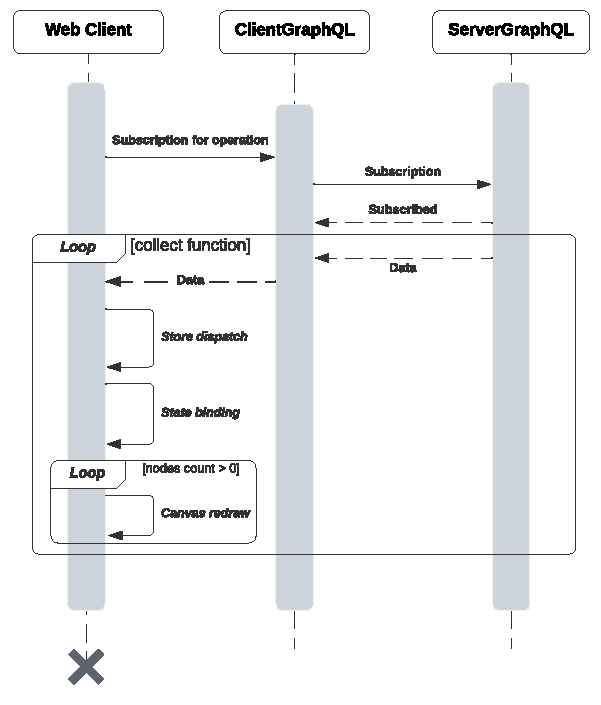
\includegraphics[scale=0.8]{imgs/Sequenza_rendering_plus.pdf}
	\caption{Diagramma di sequenza per il disegno dei nodi nel canvas}
	\label{fig:sequence-rendering-advance}
\end{figure}
Seguendo lo schema, viene effettuata una operazione di tipo \textbf{subscription} al server GraphQL per il recupero delle posizioni dei nodi. 
\lstinputlisting[float=htb, language=Kotlin, label={lst:node-subscription}, caption={Chiamata alla subscription sulla posizione dei nodi},captionpos=b,captionpos=b]{listings/SubscriptionNodes.kt}
Il \cref{lst:node-subscription} mostra la chiamata alla funzione che esegue l'operazione di \textit{subscription}. La funzione restituisce il risultato della query come un oggetto di tipo \texttt{Flow}. Quest'ultima è una classe di Kotlin che rappresenta una sequenza di valori che vengono prodotti in modo asincrono. Più nello specifico, viene restituito un \textit{cold} \texttt{Flow}. Questo significa che i dati non vengono forniti  fino a quando il flusso non viene consumato. I valori possono essere consumati in un secondo momento, come avviene nel  \cref{lst:node-subscription-collection}. Notare come in questo caso il \textit{triggering event} per l'aggiornamento dello store legato alla posizione dei nodi è proprio la funzione \texttt{collect()}.
\lstinputlisting[float=htb, language=Kotlin, label={lst:node-subscription-collection}, caption={Consumazione della subscription e aggiornamento dello store dei nodi},captionpos=b,captionpos=b]{listings/SubscriptionNodesCollection.kt}
 
 A questo punto, è necessario iscriversi ai cambiamenti di stato e richiamare la funzione \textit{redraw} del canvas, come nel \cref{lst:node-subscription-subscribe-redraw}. Il meccanismo di state binding in questo caso è reso possibile attraverso l'utlizzo della funzione \texttt{subscribe()} dello store \texttt{EnvironmentStore.store}.
\lstinputlisting[float=htb, language=Kotlin, label={lst:node-subscription-subscribe-redraw}, caption={Iscrizione agli aggiornamenti dello store e richiamo della funzione \texttt{redrawNodes()}},captionpos=b,captionpos=b]{listings/NodeSubscribeRedraw.kt}
\section{Funzionamento client web}
Il processo di \textit{bundling} menzionato in sezione \ref{section:client-web-architecture} avviene grazie all'utilizzo di \textit{Webpack}\footnote{\url{https://webpack.js.org/concepts/}}. Webpack è uno strumento
che si occupa di organizzare e quindi combinare le risorse (JavaScript, CSS, icone, font) in un numero minore di file (in questo caso solo uno, di estensione \texttt{.js}). In questo contesto non sono stati creati file CSS per la descrizione dell'aspetto delle varie componenti, dato che KVision fornisce già un certo livello di stile CSS. Inoltre, si è fatto uso di elementi che beneficiano nativamente del framework Boostrap. A prescindere da ciò, il file in output dal processo di \textit{bundling} può essere incluso nella pagina \texttt{index.html}, ottenendo il medesimo risultato che si sarebbe ottenuto includendo manualmente ogni singola risorsa.
L'esecuzione della simulazione può essere configurata appositamente con il monitor \texttt{WebUIMonitor}. Questa classe permette, in thread separati, l'avvio contemporaneo del server GraphQL e il server che ospita la pagina web che rappresenta l'interfaccia grafica.
Facendo anche riferimento alla \cref{fig:client-web-structure-graphics}, per servire la pagina principale in un browser web si è fatto utilizzo di un server \textit{Ktor} \footnote{\url{https://ktor.io/docs/create-server.html}}.
È stata configurata la \textit{route} ``\texttt{/}'' per rispondere alle richieste di tipo GET con la pagina principale \texttt{index.html}, alla quale viene impostata come risorsa statica l'artefatto \texttt{.js} ottenuto dal processo di \textit{bundling} precedentemente descritto.
\section{Verifica}
La verifica del software attraverso l'utilizzo di test automatizzati per interfacce utente, o per alcune delle loro componenti, risulta essere spesso un procedimento problematico in quanto queste tendono a essere soggette a frequenti aggiornamenti durante il loro sviluppo. In aggiunta, le \ac{UI} sono spesso soggette  a interazioni in tempo reale con l'utente, come eventi del mouse, input da tastiera e aggiornamenti dinamici. Questi aspetti rendono difficile simulare completamente il comportamento della \ac{UI} in un ambiente di test isolato, poiché è difficile riprodurre accuratamente le interazioni dell'utente durante l'esecuzione dei test. L'unica verifica che è stata effettuata avviene in tempo reale: si è interagito direttamente e in modo esaustivo con l'interfaccia durante il processo di sviluppo. Questa pratica informale ha consentito di individuare e risolvere rapidamente eventuali problemi di usabilità e comportamentali, senza la necessità di test automatizzati specifici. 
Per questi motivi, l'automatizzazione dei test sulla UI può essere complessa e richiedere risorse significative, con risultati talvolta limitati o poco pratici rispetto al testing manuale in tempo reale.

D'altro canto, per garantire la corretta rappresentazione dei nodi e l'integrità del contenuto di ciascuno di essi, sono state eseguite diverse simulazioni, nello specifico con le \textit{incarnation} \textit{protelis} e \textit{sapere}.

Si è fatto ampio ricorso al \textit{playground} GraphiQL, uno strumento che consente di consultare tutta la struttura del modello di Alchemist e le operazioni che si possono effettuare su di esso. Questo riconduce sempre al concetto di \textit{schema} delle operazioni descritto in \ref{subsection:graphql-server}. 
Dopo aver individuato il tipo di dati desiderati, sono state definite all'interno del \textit{playground} le operazioni client per verificarne l’effettivo risultato che si ottiene una volta eseguite. 
A seguito, sono state incluse all’interno delle risorse client del modulo \texttt{graphql}. 
Operando secondo questi passaggi, ogni operazione è risultata convalidata sullo \textit{schema} ancora prima della fase di compilazione, garantendo l'assenza totale di errori di sintassi durante l'esecuzione delle query o ricevimento dei dati. 





